%----------------------------------------------------------------------------------------
%    PACKAGES AND THEMES
%----------------------------------------------------------------------------------------

\documentclass{beamer}
\usepackage{graphicx}
\usepackage{ragged2e}
\usetheme{Madrid}
\usepackage{caption}
\setbeamercolor{background canvas}{bg=white}
\setbeamercolor{normal text}{fg=black}
\setbeamertemplate{footline}{%
  \leavevmode%
  \hbox{%
    \begin{beamercolorbox}[wd=\paperwidth,ht=2.25ex,dp=1ex,right]{footline}%
      \ifnum\value{framenumber}=1
        % На первом слайде ничего не показываем
        \hspace*{\fill}
      \else
        \hspace*{\fill}\insertframenumber{} / \inserttotalframenumber\hspace{0.3cm}\vspace{0.1cm}
      \fi
    \end{beamercolorbox}%
  }%
  \vskip0pt%
}
\definecolor{LightCyan}{rgb}{0.87, 0.87, 0.87}
\setbeamercolor{section in toc}{fg=black}
\setbeamercolor{subsection in toc}{fg=black}
\setbeamertemplate{caption}[numbered]
\setbeamercolor{headline}{bg=white}
\setbeamercolor{title}{fg=black}
\setbeamercolor{frametitle}{bg=white, fg=black}
\usepackage{svg}
\usepackage[T2A]{fontenc}
\usepackage[utf8]{inputenc}
\usepackage[english,russian]{babel}
\usepackage{longtable}
\usepackage{hyphenat}
\setbeamertemplate{navigation symbols}{}
\usepackage{ragged2e}
\let\raggedright=\RaggedRight
\usepackage{colortbl}
\usepackage{xcolor}
\usepackage{tikz}
\usepackage{tabularx}
\hyphenation{тех-но-ло-гия}

\begin{document}
\setbeamertemplate{frametitle}[default][center]

%----------------------------------------------------------------------------------------
%    TITLE PAGE
%----------------------------------------------------------------------------------------

\begin{frame}[plain]
    \begin{columns}[T]
        \begin{column}{0.2\textwidth}
            
\includegraphics[width=2.5cm]{assets/b_logo.png}
        \end{column}
        \begin{column}{0.8\textwidth}
            \centering
            {\footnotesize Министерство науки и высшего образования Российской Федерации\\
                Федеральное государственное автономное образовательное учреждение высшего образования\\
                <<Московский государственный технический университет
                имени Н.~Э.~Баумана
                (национальный исследовательский университет)>> \\
                (МГТУ им.~Н.~Э.~Баумана)} 
        \end{column}
    \end{columns}
    \vfill
    \centering
    {\LARGE \textbf{Метод поддержки принятия решений в рамках выполнения пошаговой инструкции, заданной в графовом формате}} \\
    \vfill
    
    \raggedleft
    {\large Группа: ИУ7-83Б} \\
    {\large Студент: Спирин Михаил Павлович} \\
    {\large Научный руководитель: Волкова Лилия Леонидовна} \\
    \vfill
    \centering
    {\small 2026 г.}
\end{frame}

%----------------------------------------------------------------------------------------
%    ОБЛАСТЬ ПРИМЕНЕНИЯ
%----------------------------------------------------------------------------------------

\begin{frame}
    \frametitle{Актуальность разработки}
    Пошаговые инструкции широко используются в различных сферах:
    \begin{itemize}
        \item[---] промышленность (монтаж и диагностика оборудования);
        \item[---] образование (обучающие материалы);
        \item[---] бытовая техника (инструкции пользователя).
    \end{itemize}
    \vfill
    Методы поддержки принятия решений позволяют в интерактивном режиме осуществлять поддержку оператора, выполняющего инструкцию.
    \vfill
    Актуальна разработка и модификация методов поддержки принятия решений оператором с учётом следующих требований.
    \begin{itemize}
        \item[---] Адаптация к возникающим нештатным ситуациям 
        \item[---] Учёт уровня экспертизы оператора в рамках домена инструкции
        \item[---] Детерминированность метода
        \item[---] Интерпретируемость результатов работы метода
    \end{itemize}
    \vfill
    % TODO: объяснить подробнее важность детерминированности
\end{frame}

%----------------------------------------------------------------------------------------
%    ЦЕЛЬ И ЗАДАЧИ
%----------------------------------------------------------------------------------------

\begin{frame}{\centering Цель и задачи работы}
    \textbf{Цель работы}~---~разработка метода поддержки принятия решений при выполнении пошаговой инструкции, заданной в графовом формате.
    
    \vfill
    \textbf{Задачи:}
    \begin{itemize}
        \item[---] рассмотреть и сравнить известные методы, которые могут быть применены для поддержки принятия решений;
        \item[---] формализовать постановку задачи разработки метода поддержки принятия решений на основе графового представления инструкции;
        \item[---] разработать метод поддержки принятия решений и реализовать его программно;
        \item[---] провести исследование эффективности предложенного метода, включая сравнение классического и модифицированного МАИ по временным затратам эксперта и качеству выдаваемых рекомендаций.
    \end{itemize}
\end{frame}

%----------------------------------------------------------------------------------------
%    ГРАФОВЫЙ ФОРМАТ ОПИСАНИЯ ИНСТРУКЦИЙ
%----------------------------------------------------------------------------------------

\begin{frame}
    \frametitle{Графовый формат описания инструкций}
    
    \begin{columns}
        \begin{column}{0.3\textwidth}
            \begin{itemize}
                \item Используется специальный гибридный графовый формат описания инструкции [1].
                \item Хранит:
                \begin{itemize}
                    \item[---] сущности
                    \item[---] состояния контекста
                    \item[---] переходы между состояниями
                \end{itemize}
            \end{itemize}
        \end{column}
        
        \begin{column}{0.7\textwidth}
            \begin{figure}[H]
                \centering
                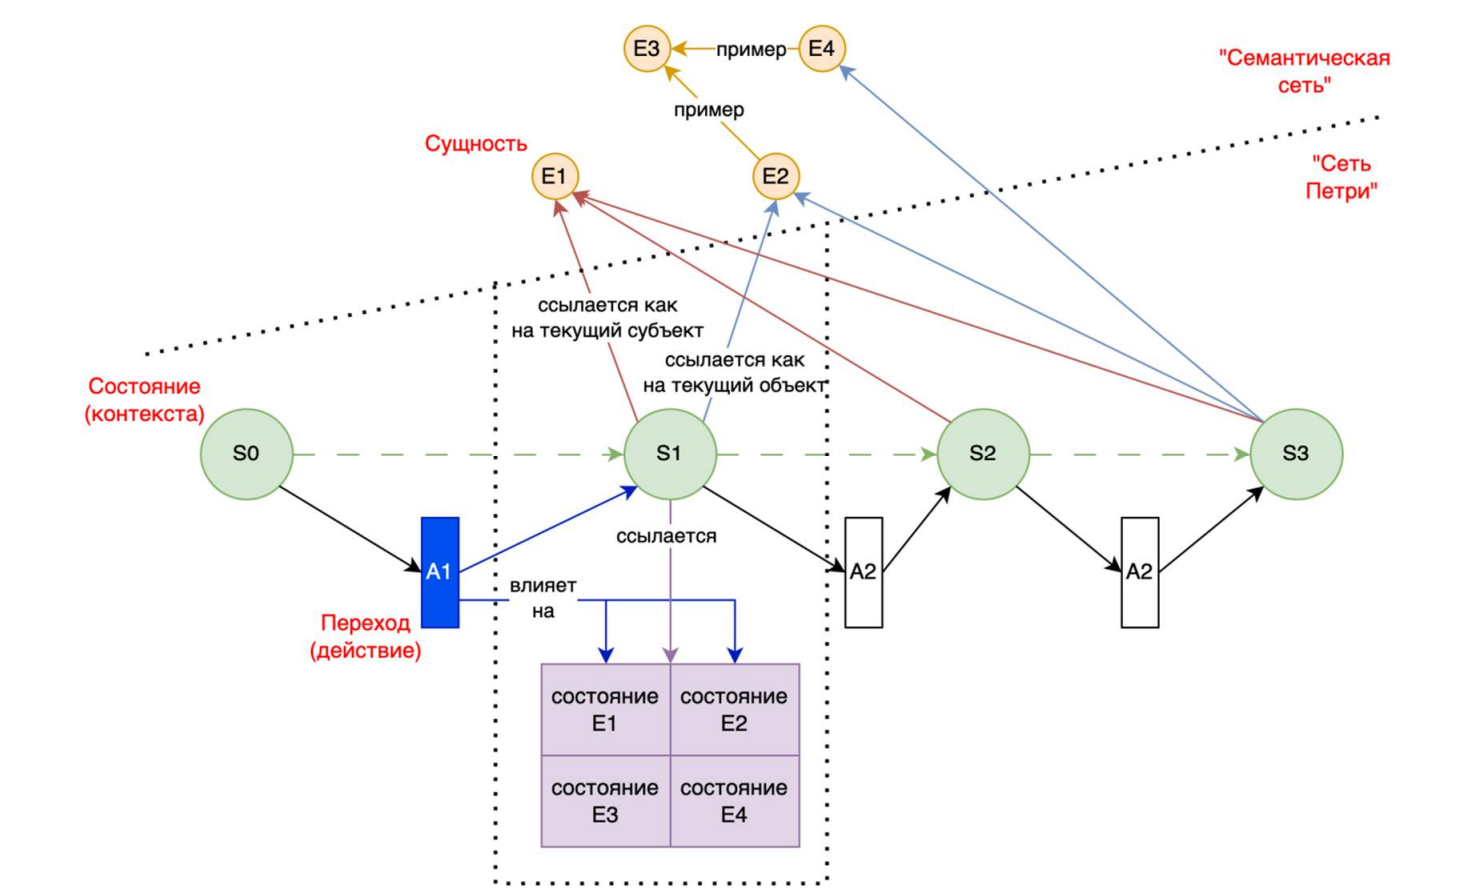
\includegraphics[width=\textwidth]{assets/graph.png}
            \end{figure}
        \end{column}
    \end{columns}
{\tiny \vfill
[1] Кормановский М.В., Волкова Л.Л. Графовый формат представления пошаговых русскоязычных инструкций: действия, сущности, контекст // Первый Евразийский конгресс лингвистов. — М.:
Институт языкознания РАН, 2025. — С. 391--393.}
    
\end{frame}

%----------------------------------------------------------------------------------------
%    ФОРМАЛИЗАЦИЯ ЗАДАЧИ
%----------------------------------------------------------------------------------------

\begin{frame}
    \frametitle{Формализация задачи}
    Граф инструкции $ G = (V, E) $, где:
    \begin{itemize}
        \item[---] $ V = S \cup A $ --- множество вершин;
        \item[---] $S$ ---  множество состояний;
        \item[---] $A$ ---  множество действий;
        \item[---] $ E \subseteq S \times A \cup A \times S $ --- множество дуг.
    \end{itemize}
    \vspace{0.2cm} %\{s_1, s_2, \dots, s_n\}
    Каждое состояние $ s_i \in S $ характеризуется названием состояния, описание, типом (начальным, промежуточным, конечным, ошибочным), состоянием объектов в данном состоянии.
    \vspace{0.2cm}

    Требуется построить отображение:
    \[
        F: S \times A \to R^+,
    \]
    где каждой паре состояния $s_i \in S$ и действия $a_i \in A$ ставится в соответствие кортеж рекомендаций $r \in R^+$.
\end{frame}

%----------------------------------------------------------------------------------------
%    ПРЕДЛАГАЕМЫЙ МЕТОД (A0)
%----------------------------------------------------------------------------------------

\begin{frame}
    \frametitle{Предлагаемый метод}
    
    
    \begin{columns}
        \begin{column}{0.6\textwidth}
            \begin{figure}[H]
                \centering
                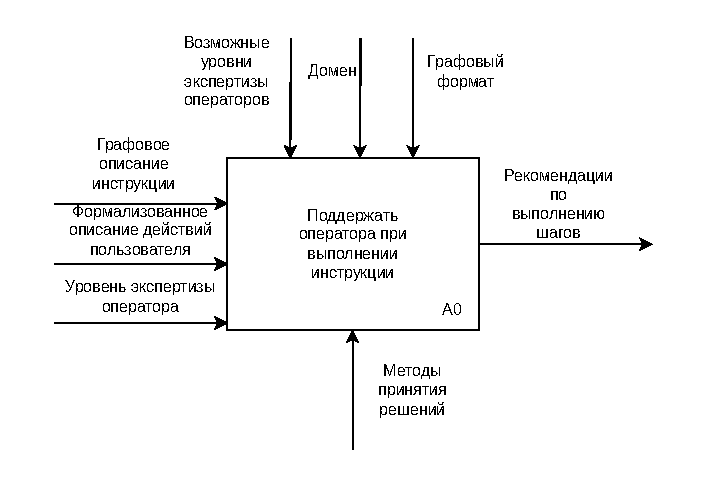
\includegraphics[width=\textwidth]{assets/idef1.pdf}
            \end{figure}
        \end{column}
        
        \begin{column}{0.4\textwidth}
            {\small
        \textbf{Ограничения}.
        \begin{itemize}
            \item[---] Инструкция задана в виде ориентированного графа без циклов.
            \item[---] Эксперт задаёт оценки рекомендациям по критериям по шкале от 0 до 1. 
            Для новых инструкций проводится настройка меток и оценок.
            \item[---] Аварийные сценарии предварительно описаны в виде отдельных графов и описаны метками.
        \end{itemize}
            }
        \end{column}
    \end{columns}
\end{frame}
    
%----------------------------------------------------------------------------------------
%    ПРЕДЛАГАЕМЫЙ МЕТОД (A1)
%----------------------------------------------------------------------------------------

\begin{frame}
    \frametitle{Предлагаемый метод, детализация}
    \begin{figure}[H]
        \centering
        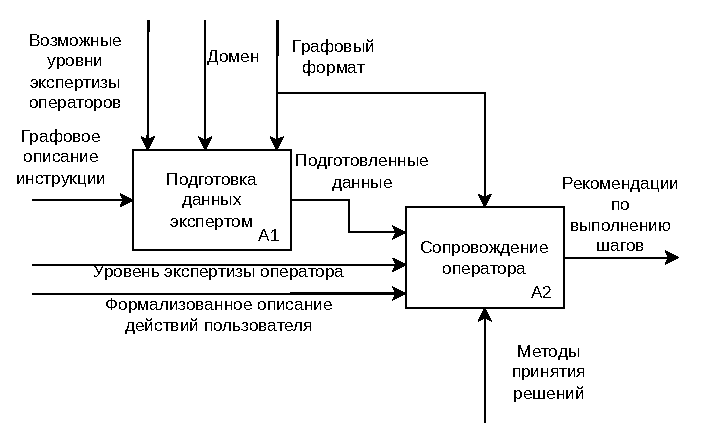
\includegraphics[width=\textwidth]{assets/idef0_x.pdf}
    \end{figure}
\end{frame}

%----------------------------------------------------------------------------------------
%    СРАВНЕНИЕ МЕТОДОВ 
%----------------------------------------------------------------------------------------
\begin{frame}
    \frametitle{Сравнение методов теории принятия решений}
    Критерии:
    \begin{itemize}
        \item[---] \textbf{K1} --- требование к числовым или категориальным данным;
        
        \item[---] \textbf{K2} --- учёт субъективных факторов;
        
        \item[---] \textbf{K3} --- поддержка неполных данных;
        
        \item[---] \textbf{К4} --- устойчивость к изменениям критериев и входных данных;
        
        \item[---] \textbf{К5} --- наличие ранжирования.
        
    \end{itemize}
    \begin{center}
        \begin{tabular}{|c|c|c|c|c|c|}
            \hline
            \textbf{Метод} & \textbf{К1} & \textbf{К2} & \textbf{К3} & \textbf{К4} & \textbf{К5} \\
            \hline
            ELECTRE & Смешанные & Да & Да & Высокая & Частично \\
            \hline
            TOPSIS & Числовые & Нет & Нет & Средняя & Да \\
            \hline
            \rowcolor{lightgray} МАИ & Категориальные & Да & Частично & Средняя & Да \\
            \hline
        \end{tabular}
    \end{center}
\end{frame}

%----------------------------------------------------------------------------------------
%    МЕТОД АНАЛИЗА ИЕРАРХИЙ (МАИ)
%----------------------------------------------------------------------------------------
\begin{frame}
    \frametitle{Профили экспертизы}
    \small 
    На основе выбранного метода предлагается ввести различные профили экспертизы оператора для достижения лучших результатов.
    
    Выбор профиля влияет на веса критериев, и, следовательно, на выводимые рекомендации.
    
    \textbf{Примеры} возможных весов критериев для разных уровней экспертизы:
    
    % TODO: тут коцые цифры на абсциссе
    \begin{figure}[H]
        \centering
        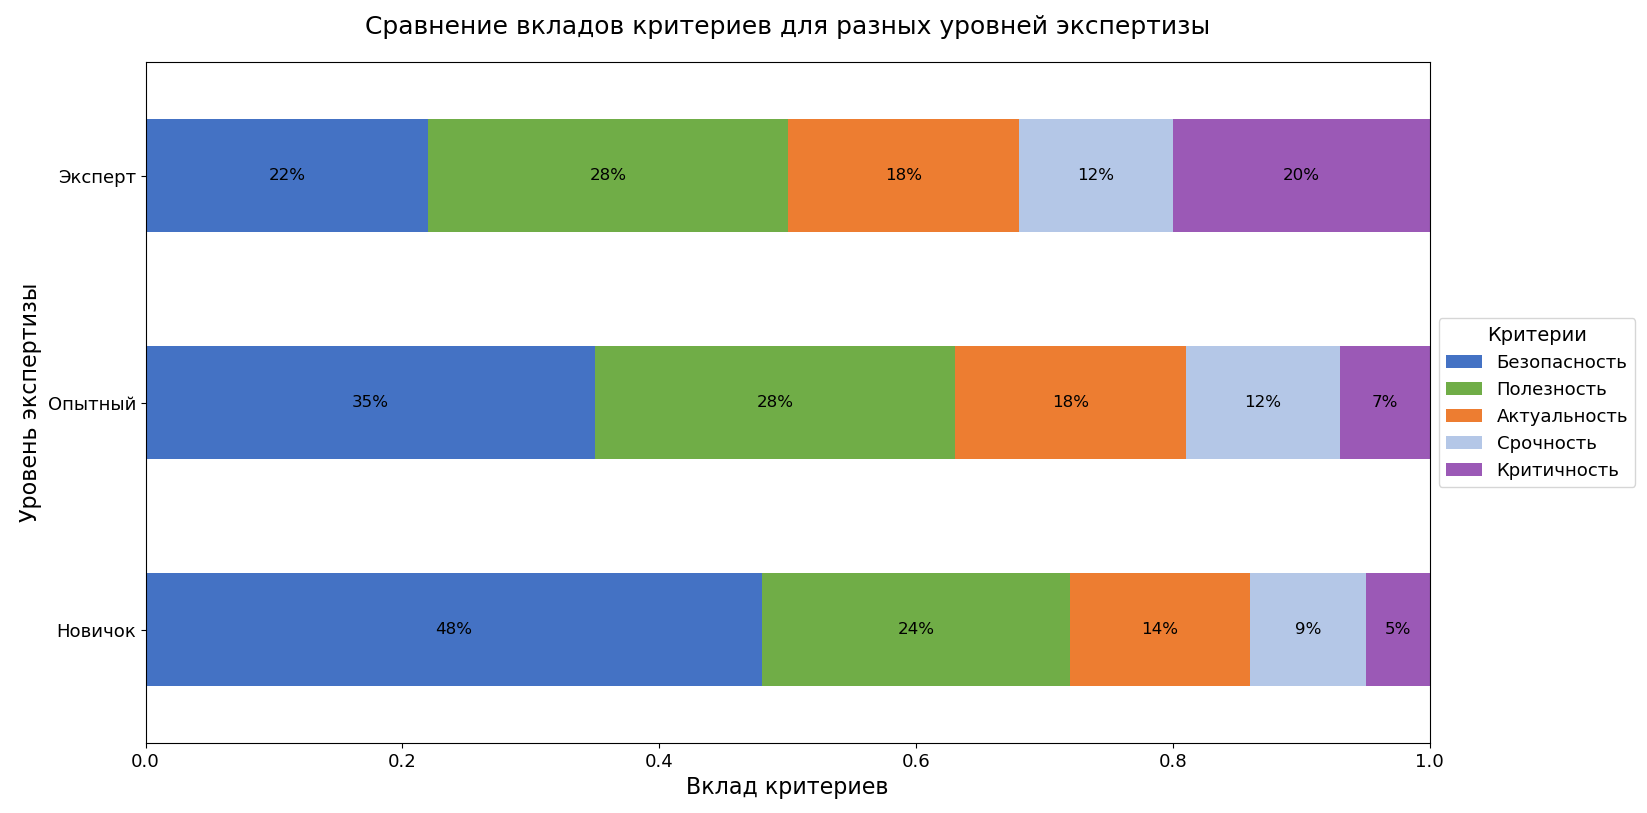
\includegraphics[width=0.97\textwidth]{assets/expertise.png}
    \end{figure}
\end{frame}

\begin{frame}
    \frametitle{Метод анализа иерархий (МАИ)}
    \textbf{Особенности МАИ~[2].}
    \begin{itemize}
        \item[---] Построение иерархии: цель, критерии, альтернативы.
        \item[---] Попарные сравнения элементов по шкале Саати (1---9).
        \item[---] Вычисление весов на основе матриц попарных сравнений.
        \item[---] Вычисляется отношение согласованности (CR). Если CR < 0.1 — суждения эксперта считаются согласованными.
    \end{itemize}
    \textbf{Недостатки.}
    \begin{itemize}
        \item[---] Значительная зависимость от субъективной оценки эксперта.
        \item[---] Квадратичный рост числа сравнений --- для \(n\) элементов требуется \(\frac{n(n-1)}{2}\) попарных сравнений, что делает метод трудоёмким для задач с большим числом альтернатив.
        \item[---] Отсутствие возможности явно работать с нечёткой или вероятностной информацией.
    \end{itemize}
    \vspace{0.5cm}
{\tiny [2] Saaty T. L. The Analytic Hierarchy Process: Planning, Priority Setting, Resource Allocation. — New York : McGraw-Hill, 1980. — 287 с.}
\end{frame}

\begin{frame}
    \frametitle{Предлагаемая модификация МАИ}
    {\small 
    Модификация решает проблему высокой трудоёмкости разметки попарных сравнений для задач с большим числом альтернатив.

    \textbf{Ключевые особенности:}
    \begin{itemize}
    \item[---] Альтернативы объединяются в \textbf{группы}. \textbf{Элементами} группы могут быть группы или альтернативы. Все группы непустые. 
    \item[---] Попарные сравнения проводятся только между элементами одной группы.
    \item[---] Если один элемент группы приоритетнее другого, то все его элементы тоже считаются более приоритетными.
    % \item[---] Отбор жадный --- рассматриваем только потенциальные лучшие альтернативы. 
    \end{itemize}

    \begin{columns}[T]
        \begin{column}{0.55\textwidth}
            \textbf{Ранжирование.} Для поиска наиболее подходящей альтернативы ранжируются элементы группы аналогично стандартному МАИ, после чего поиск рекурсивно продолжается в лучшем элементе изначальной группы.
        \end{column}
        \begin{column}{0.4\textwidth}
            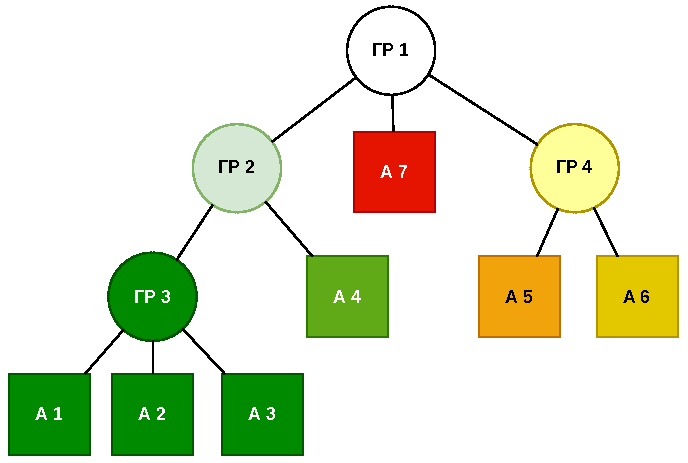
\includegraphics[width=\textwidth]{assets/tree.pdf}
        \end{column}
    \end{columns}
    
    }

\end{frame}

%----------------------------------------------------------------------------------------
%    АЛГОРИТМ ОПРЕДЕЛЕНИЯ ВЕСОВ КРИТЕРИЕВ
%----------------------------------------------------------------------------------------

\begin{frame}
\frametitle{Алгоритм вычисления весов критериев}
    \textbf{Вход:} список критериев \(C = \{c_1,\dots,c_n\}\), матрица попарных сравнений \(A\) (размер \(n \times n\)), где \(a_{ij}\) --- степень превосходства критерия \(c_i\) над \(c_j\) по шкале Саати.
    
    \textbf{Алгоритм.}
    \begin{enumerate}
        \item[---] Для каждой строки \(i\) матрицы попарных сравнений вычислить геометрическое среднее:
            $g_i = \left( \prod_{j=1}^{n} a_{ij} \right)^{1/n}.$
        \item[---] Нормализовать: \(w_i = g_i / \sum_{k=1}^{n} g_k\).
        \item[---] Вычислить вектор \(A_w\): \((A_w)_i = \sum_{j=1}^{n} a_{ij} w_j\).
        \item[---] Найти \(\lambda_{\max} = \frac{1}{n} \sum_{i=1}^{n} \frac{(A_w)_i}{w_i}\).
        \item[---] Индекс согласованности: \(CI = \frac{\lambda_{\max} - n}{n-1}\).
        \item[---] Отношение согласованности: \(CR = CI / RI\), где \(RI\) --- случайный индекс для матрицы размером \(n\) (таблица Саати).
        \item[---] Если \(CR < 0.1\), матрица считается согласованной.
    \end{enumerate}
    \textbf{Выход:} вектор весов \(w = (w_1,\dots,w_n)\), индекс согласованности \(CI\), отношение согласованности \(CR\).
\end{frame}

%----------------------------------------------------------------------------------------
%    АЛГОРИТМ РАНЖИРОВАНИЯ РЕКОМЕНДАЦИЙ
%----------------------------------------------------------------------------------------


% TODO: перепроверить тут формулу, возможно стоит упростить
\begin{frame}
    \frametitle{Алгоритм ранжирования рекомендаций}
    \textbf{Вход:} набор меток \(L\) с рекомендациями \(R_a = \{r_1,\dots,r_m\}\), \(m\) --- количество рекомендаций, связанных с действием, веса критериев \(w_c\), количество искомых наиболее подходящих рекомендаций \(n\), количество критериев \(k\).
    \vspace{0.2cm}

    \textbf{Алгоритм:}
    \begin{enumerate}
        \item[---] Инициализировать пустой список оценок \(S\).
        \item[---] Для каждой рекомендации \(r_i\):
        \begin{itemize}
                \item[---] получить оценки по критериям \(s_{i,c}\) из конфигурации;
                \item[---] вычислить интегральную оценку \(S_i = \sum_{c=1}^{k} w_c \cdot s_{i,c}\).
            \end{itemize}
            \item[---] Вычислить сумму \(T = \sum_{i=1}^{m} S_i\).
            \item[---] Провести нормализацию \(\tilde{S}_i = S_i / T\).
        \item[---] Отсортировать рекомендации по убыванию \(\tilde{S}_i\).
        \item[---] Вернуть \(n\) лучших элементов с их оценками.
    \end{enumerate}
    \vspace{0.2cm}
    \textbf{Выход:} список рекомендаций, отсортированный по убыванию нормализованной оценки.
\end{frame}


%----------------------------------------------------------------------------------------
%    ОБРАБОТКА АВАРИЙНЫХ СЦЕНАРИЕВ
%----------------------------------------------------------------------------------------

% \begin{frame}
%     \frametitle{Обработка аварийных сценариев}
%     \textbf{Алгоритм.}
%     \begin{enumerate}
%         \item[---] Получить ключевые слова из меток действия.
%         \item[---] Найти сценарии с пересекающимися тегами.
%         \item[---] Предложить пользователю выбор.
%         \item[---] Загрузить и выполнить аварийный граф.
%         \item[---] Вернуться к основному сценарию (при необходимости).
%     \end{enumerate}
% \end{frame}

\begin{frame}    
\frametitle{Алгоритм модификации МАИ}
{\footnotesize
\textbf{Вход}: множество альтернатив \(A = \{a_1, a_2, \dots, a_m\}\), множество групп и для каждой группы \(G_k\) --- список ее элементов $e_{k}$, матрицы попарных сравнений элементов групп, $n$ --- количество искомых лучших рекомендаций. \textbf{Выход:} список из $n$ лучших рекомендаций.

% \textbf{Шаг 1. Агрегирование весов корневых элементов.}

% Для каждого критерия \(c\) вычисляются локальные приоритеты элементов корневой группы \(w_{c,\text{root}}(e)\). Затем веса агрегируются с учётом глобальных весов критериев \(w_c\):
% \[
% W_{\text{root}}(e) = \sum_{c} w_c \cdot w_{c,\text{root}}(e).
% \]

% \textbf{Шаг 2. Рекурсивный отбор лучших альтернатив.}

Для набора элементов \(children(G)\) группы \(G\):
% TODO: тут можно получить по голове
\begin{enumerate}
    \item Вычисляются локальные приоритеты \(w_{c,G}(e)\) по каждому критерию аналогично стандартному МАИ.
    \item Определяются глобальные приоритеты:
    \[
    W_G(e) = \sum_{c} w_c \cdot w_{c,G}(e).
    \]
    \item Элементы сортируются по убыванию \(W_G(e)\).
    \item Пока не набрано \(N\) альтернатив, для первого нерассмотренного элемента:
        \begin{itemize}
            \item Если элемент --- альтернатива, она добавляется в результат.
            \item Если элемент --- группа, процедура применяется к ней рекурсивно.
        \end{itemize}
    \item Вернуть список найденных лучших альтернатив.
\end{enumerate}
}
\end{frame}

\begin{frame}
    
\frametitle{Обработка аварийных сценариев}
\textbf{Вход:} действие \(a\), которое оператор отказался выполнять, текущий контекст (метки действия).

\textbf{Алгоритм.}
\begin{enumerate}
    \item[---] Получить ключевые слова из всех меток действия \(K_a\).
    \item[---] Для каждого аварийного сценария \(e\) из конфигурации: если множество меток сценария \(T_e\) пересекается с \(K_a\), добавить сценарий в список доступных.
    \item[---] Предложить оператору выбрать сценарий из списка.
    \item[---] Если выбор сделан:
    \begin{itemize}
        \item[---] загрузить граф сценария из файла;
        \item[---] начать его выполнение;
        \item[---] по завершении вернуть флаг \(return\_to\_original\) из конфигурации сценария.
    \end{itemize}
    \item[---] Иначе продолжить основной сценарий.
    \end{enumerate}
\textbf{Выход:} флаг необходимости возврата к основному сценарию.
\end{frame}
%----------------------------------------------------------------------------------------
%    ДИАГРАММА КОМПОНЕНТОВ
%----------------------------------------------------------------------------------------

\begin{frame}
    \frametitle{Структура ПО}
    \begin{figure}[H]
        \centering
        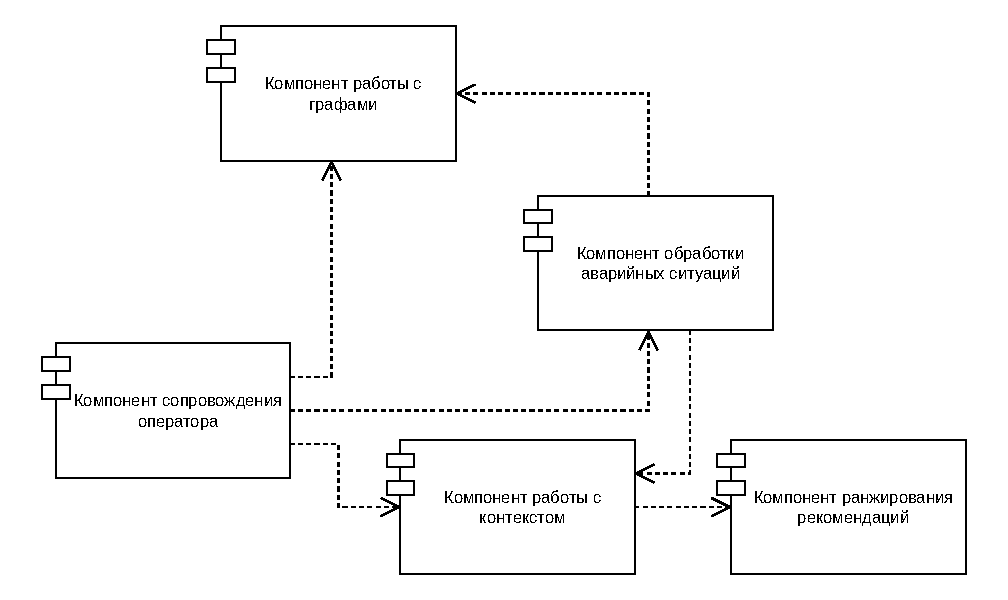
\includegraphics[width=\textwidth]{assets/comp_diagram.pdf}
    \end{figure}
\end{frame}

\begin{frame}
    \frametitle{Структура ПО}
    \begin{figure}[H]
        \centering
        
\includegraphics[width=1.0\textwidth]{assets/sequence.png}
    \end{figure}
\end{frame}

%----------------------------------------------------------------------------------------
%    ПРОФИЛИ ЭКСПЕРТИЗЫ
%----------------------------------------------------------------------------------------

% \begin{frame}
%     \frametitle{Профили экспертизы}
%     Функциональность разработанного метода позволяет выбрать профиль экспертизы оператора.
%     Выбор профиля влияет на веса критериев и приоритет рекомендаций.
    
%     Примеры возможных весов критериев в зависимости от уровня экспертизы оператора:
%     % TODO: можно тепловую карту здесь сделать, было бы красиво (еще лучше "гистограмму с накоплением + еще что то" (см пикчу). В excel это линейчатая нормированная с накоплением)
%     % TODO: добавить мотивацию
% \end{frame}

%----------------------------------------------------------------------------------------
%    ЗАВИСИМОСТЬ ВРЕМЕНИ ОТ КОЛИЧЕСТВА АЛЬТЕРНАТИВ
%----------------------------------------------------------------------------------------

% \begin{frame}
%     \frametitle{Сравнение временных затрат}
%     % \begin{figure}[H]
%     %     \centering
%     %     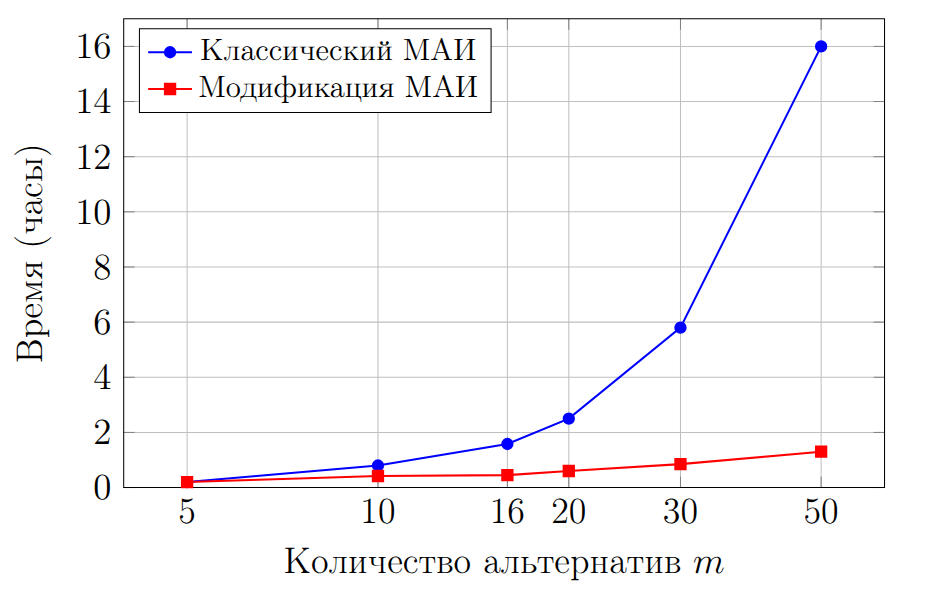
\includegraphics[width=0.8\textwidth]{assets/time_graph.png}
%     % \end{figure}
%     % \vspace{-0.3cm}
%     \tiny
%     \begin{center}
%         \begin{tabular}{|c|c|c|c|}
%             \hline
%             \textbf{Альтернатив} & \textbf{Классический (ч)} & \textbf{Модификация (ч)} & \textbf{Ускорение} \\
%             \hline
%             5 & 0.20 & 0.20 & 1.0× \\
%             \hline
%             10 & 0.80 & 0.42 & 1.9× \\
%             \hline
%             16 & 1.58 & 0.45 & 3.5× \\
%             \hline
%             20 & 2.50 & 0.60 & 4.2× \\
%             \hline
%             30 & 5.80 & 0.85 & 6.8× \\
%             \hline
%             50 & 16.0 & 1.30 & 12.3× \\
%             \hline
%             100 & 64.0 & 2.60 & 24.6× \\
%             \hline
%         \end{tabular}
%     \end{center}
% \end{frame}
\begin{frame}
    \frametitle{План исследования эффективности метода}

    {\small
    \textbf{Исследование 1. Сравнение временных затрат классического и модифицированного МАИ}

        \textbf{Цель:} определить среднее время разметки одного попарного сравнения и сравнить трудозатраты эксперта при разном количестве альтернатив для двух реализаций МАИ.
        
        \textbf{Особенности:}
        \begin{itemize}
            \item[---] Эксперт работает сеансами длиной до 2 часов
            \item[---] Количество попарных сравнений составляет от 5 до 100
            \item[---] Фиксация времени подготовки (5 мин) и чистого времени разметки
        \end{itemize}
    
    \textbf{Исследование 2. Оценка качества рекомендаций до и после настройки весов}

        \textbf{Цель:} определить влияние экспертной настройки весов критериев на качество выдаваемых рекомендаций.
        
        \textbf{Параметры:}
        \begin{itemize}
            \item[---] 3 сценария: приготовление кофе, жарка яичницы, варка компота
            \item[---] Оценка рекомендаций по шкале от 1 до 3 (1 худшая, 3 лучшая)
            \item[---] Настройка весов в режиме отладки и повторная оценка
        \end{itemize}
    }
\end{frame}

%----------------------------------------------------------------------------------------
%    ЗАВИСИМОСТЬ ВРЕМЕНИ ОТ КОЛИЧЕСТВА СРАВНЕНИЙ
%----------------------------------------------------------------------------------------
% TODO: возможно гистограмма
% TODO: можно даже объединить со следующим слайдом
\begin{frame}
    \frametitle{Зависимость времени работы эксперта от количества сравнений}
    
    \begin{figure}[H]
        \centering
        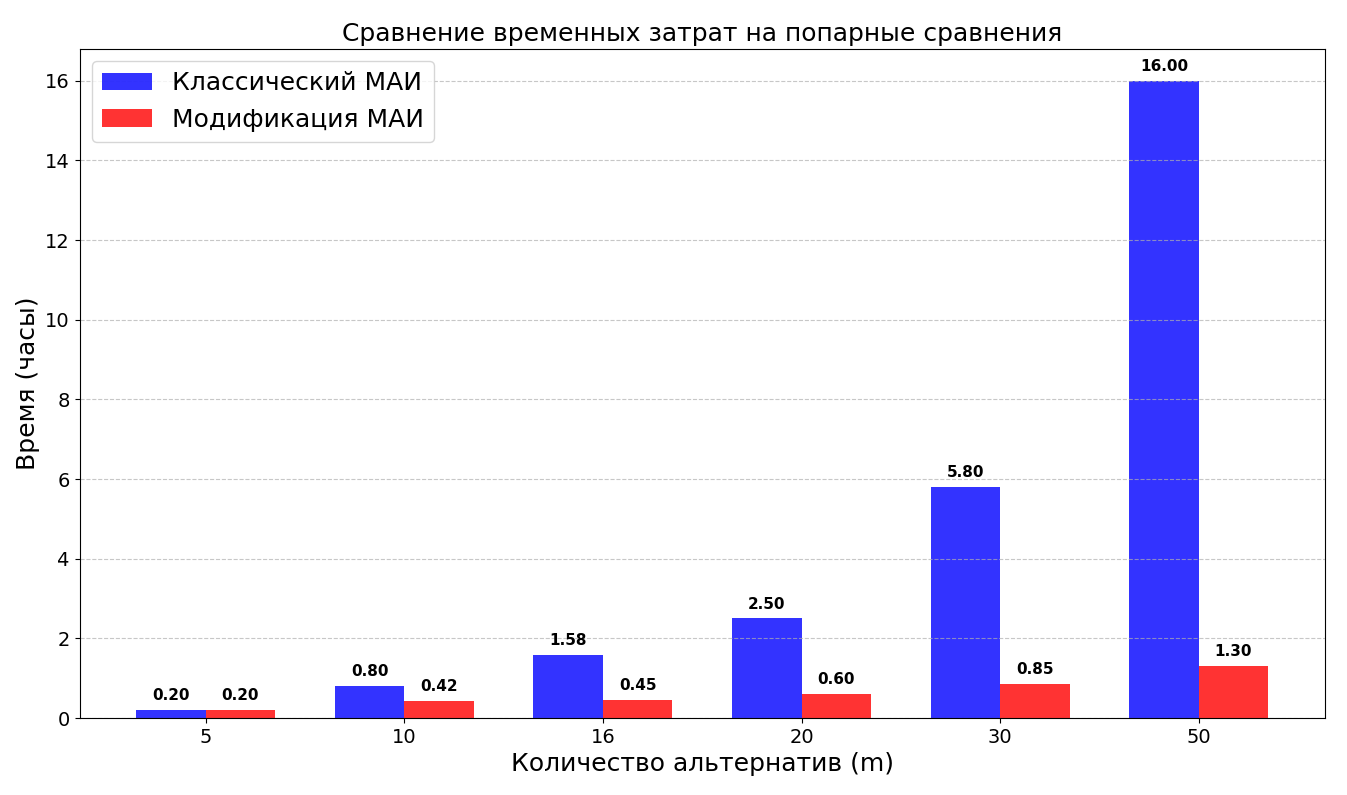
\includegraphics[width=0.75\textwidth]{assets/time_comparison.png}
    \end{figure}
    {\small
    \begin{itemize}
        \item[---] Среднее время разметки одного попарного сравнения --- 42 секунды.
        \item[---] Время разметки сравнений двух методов сравнимо до 10 альтернатив.
        \item[---] Модификация МАИ требует в 10---25 раз меньше времени при 50---100 альтернативах.
    \end{itemize}
    }
    % \vspace{-0.3cm}
    % \tiny
    % \begin{center}
    %     \begin{tabular}{|c|c|c|c|}
    %         \hline
    %         \textbf{Количество сравнений} & \textbf{Чистое время (мин)} & \textbf{Общее время (мин)} & \textbf{Сеансов} \\
    %         \hline
    %         10 & 7 & 12 & 1 \\
    %         \hline
    %         28 & 20 & 25 & 1 \\
    %         \hline
    %         45 & 32 & 37 & 1 \\
    %         \hline
    %         61 & 43 & 48 & 1 \\
    %         \hline
    %         100 & 70 & 75 & 1 \\
    %         \hline
    %         165 & 116 & 126 & 2 \\
    %         \hline
    %         495 & 347 & 367 & 4 \\
    %         \hline
    %         1225 & 858 & 898 & 8 \\
    %         \hline
    %     \end{tabular}
    % \end{center}
\end{frame}


% \begin{frame}
%     \frametitle{Выводы}
%     \begin{itemize}
%         \item[---] Среднее время разметки одного попарного сравнения составляет 42 секунды.
%         \item[---] Необходимое время для разметки сравнений двух методов сравнимо до 10 альтернатив.
%         \item[---] Модификация МАИ требует в 10---25 раз меньше времени при 50---100 альтернативах.
%     \end{itemize}
% \end{frame}

%----------------------------------------------------------------------------------------
%    КАЧЕСТВО РЕКОМЕНДАЦИЙ ДО И ПОСЛЕ НАСТРОЙКИ
%----------------------------------------------------------------------------------------

% TODO: может визуализация
% TODO: сделать постановку обоих исследований в один слайд перед ними
\begin{frame}
    \frametitle{Оценка качества рекомендаций}
    \small
    \setlength{\tabcolsep}{3pt}
    \begin{table}[H]
        \centering
        \begin{tabular}{|p{0.25\textwidth}|p{0.22\textwidth}|p{0.25\textwidth}|p{0.18\textwidth}|}
            \hline
            \textbf{Сценарий} & \textbf{До настройки} & \textbf{После настройки} & \textbf{Изменение} \\
            \hline
            Приготовление кофе & 2.2 & 2.5 & +0.3 \\
            \hline
            Жарка яичницы & 2.0 & 2.5 & +0.5 \\
            \hline
            Варка компота & 2.1 & 2.7 & +0.6 \\
            \hline
            \textbf{Среднее} & \textbf{2.1} & \textbf{2.57} & \textbf{+0.47} \\
            \hline
        \end{tabular}
    \end{table}
    \begin{itemize}
        \item[---] Базовая конфигурация весов рекомендаций требует доработки экспертом для достижения высокого качества (2.1 из 3.0).
        \item[---] После настройки средняя оценка качества повысилась до 2.57, что свидетельствует об эффективности предложенного механизма.
        \item[---] Рекомендуется проводить настройку весов перед промышленным использованием системы для новой предметной области.
    \end{itemize}
\end{frame}

% \begin{frame}
%     \frametitle{Выводы}
%     \begin{itemize}
%         \item[---] Базовая конфигурация весов рекомендаций требует доработки экспертом для достижения высокого качества (2.1 из 3.0).
%         \item[---] После настройки средняя оценка качества повысилась до 2.57, что свидетельствует об эффективности предложенного механизма.
%         \item[---] Рекомендуется проводить настройку весов перед промышленным использованием системы для новой предметной области.
%     \end{itemize}
% \end{frame}


%----------------------------------------------------------------------------------------
%    ЗАКЛЮЧЕНИЕ
%----------------------------------------------------------------------------------------

\begin{frame}{\centering Заключение}
    \textbf{Цель работы достигнута:} разработан метод поддержки принятия решений при выполнении пошаговой инструкции, заданной в графовом формате.
    
    \vfill
    
    \textbf{Решены следующие задачи:}
    \begin{itemize}
        \item[---] рассмотрены и сравнены известные методы, которые могут быть применены для поддержки принятия решений;
        \item[---] формализована постановка задачи разработки метода поддержки принятия решений на основе графового представления инструкции;
        \item[---] разработан описанный метод;
        \item[---] разработано программное обеспечение, реализующее данный метод;
        \item[---] проведено исследование эффективности предложенного метода.
    \end{itemize}
\end{frame}

%----------------------------------------------------------------------------------------
%    ДАЛЬНЕЙШЕЕ РАЗВИТИЕ
%----------------------------------------------------------------------------------------

% TODO: название слайда?
\begin{frame}
    \frametitle{Дальнейшее развитие}
    \begin{itemize}
        \item[---] Добавление функциональности отслеживания инвентаря.
        \item[---] Интеграция с голосовыми помощниками.
        \item[---] Поддержка автоматического извлечения инструкций в графовом формате из текстовых описаний.
        \item[---] Разработка веб-интерфейса для удалённого использования.
        \item[---] Интеграция с системами умного дома для автоматического контроля выполнения шагов.
        \item[---] Добавление функции совместного выполнения инструкций несколькими пользователями.
    \end{itemize}
    \textbf{Публикационная активность}
     Принята к печати публикация в сборник материалов национальной научно-практической конференции ФППИиИП-2026 (РИНЦ).
\end{frame}
\end{document}

% TODO: увеличить таблицы